\section{Teste de localização com smartphone}
\label{sec:teste-smarphone}

Para verificar a capacidade do sensores de localizar contextualmente um
dispositivo móvel, smartphone, foi utilizado. Este foi posicionado em duas salas
diferentes, em cada uma das salas foi executada uma captura de 10 minutos. Para
que houvesse tráfego na rede o dispositivo móvel foi configurado para receber um
stream de vídeo no aplicativo \emph{Netflix}.

\begin{figure}[htb]
	\caption{\label{fig-planta-baixa}Ambiente de teste}
	\begin{center}
		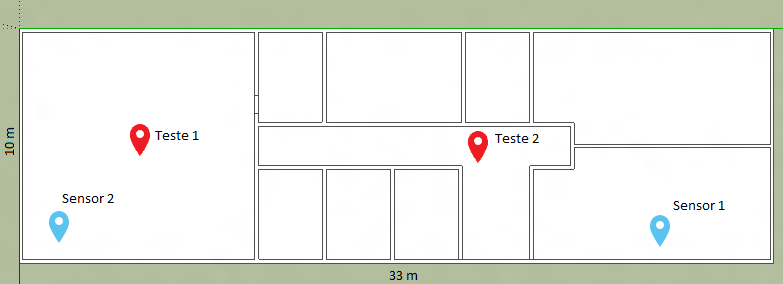
\includegraphics[width=1\textwidth]{060-testes/data-analisis/planta-baixa-smartphone.png}
	\end{center}
	\legend{Fonte: Elaborada pelo autor}
	\nota[Em azul]{Sensores da aplicação}%
	\nota[Em vermelho]{Pontos do dispositivo teste}%
\end{figure}


A captura foi realizada utilizando a ferramenta TShark da mesma maneira que é utilizada no
aplicativo. A descrição deste modo de operação pode ser encontrada no capítulo de construção.


Para o primeiro caso o dispositivo estava na mesma sala do sensor número 2 que é a maior
sala do prédio com 12  metros de comprimento por 10 metros  De largura. neste caso foram
capturados 157736 pacotes totalizando 9.7 megabytes pelo sensor 1 21974 pacotes totalizando
1.9 megabytes de captura pelo sensor 2.

No segundo teste o dispositivo móvel estava posicionado no corredor fora da sala do sensor 1
e distante do sensor 2.  neste teste o sensor 1 capturou 103555 pacotes totalizando 6.4 megabytes
de captura e o sensor 2 capturou 22635 pacotes totalizando 2 megabytes de captura

Posteriormente os arquivos de captura foram analisados com a ferramenta
\emph{Ron’s Editor} para que um sumário fosse construído.

\begin{figure}[htb]
	\label{mg4-noise}
	\centering
	\begin{minipage}{0.49\textwidth}
	\centering
		\caption{\label{fig-mg4-noise-t1}Captura total (noise) - Teste 1}
		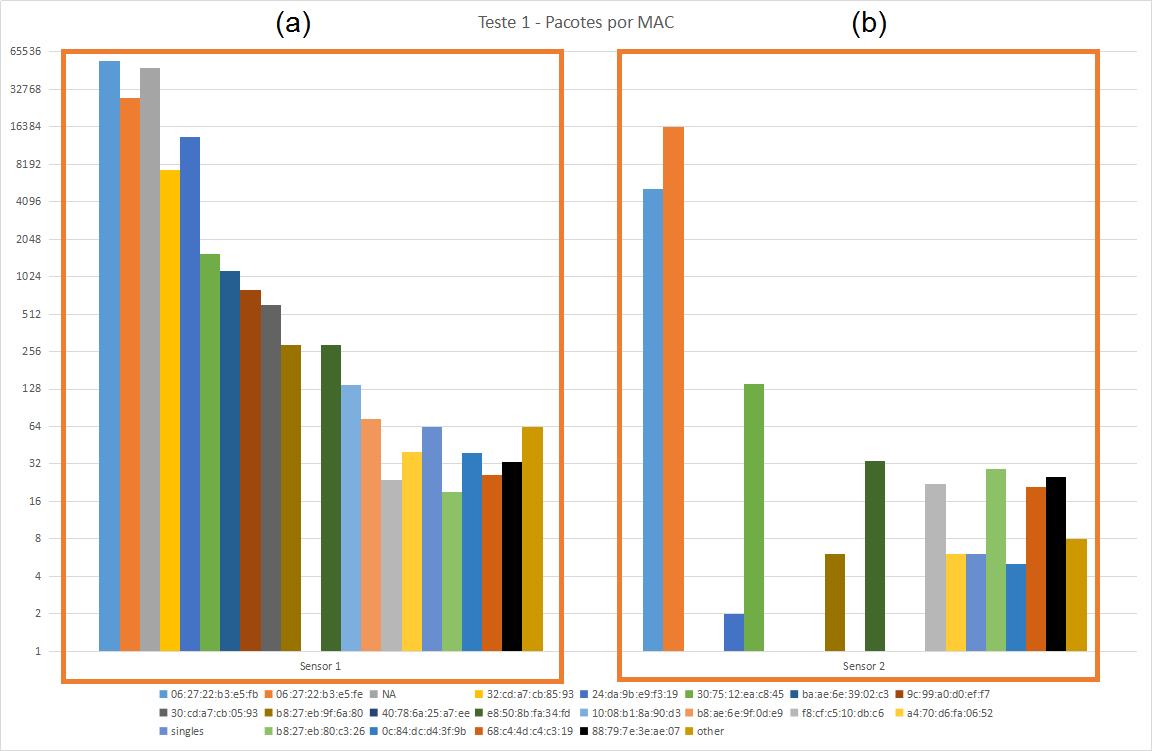
\includegraphics[width=1\textwidth]{060-testes/data-analisis/distance-mg4plus-netflix/Teste1.png}
		\legend{Fonte: Elaborada pelo autor}
	\end{minipage}
	\hfill
	\begin{minipage}{0.49\textwidth}
	\centering
		\caption{\label{fig-mg4-noise-t2}Captura total (noise) - Teste 2}
		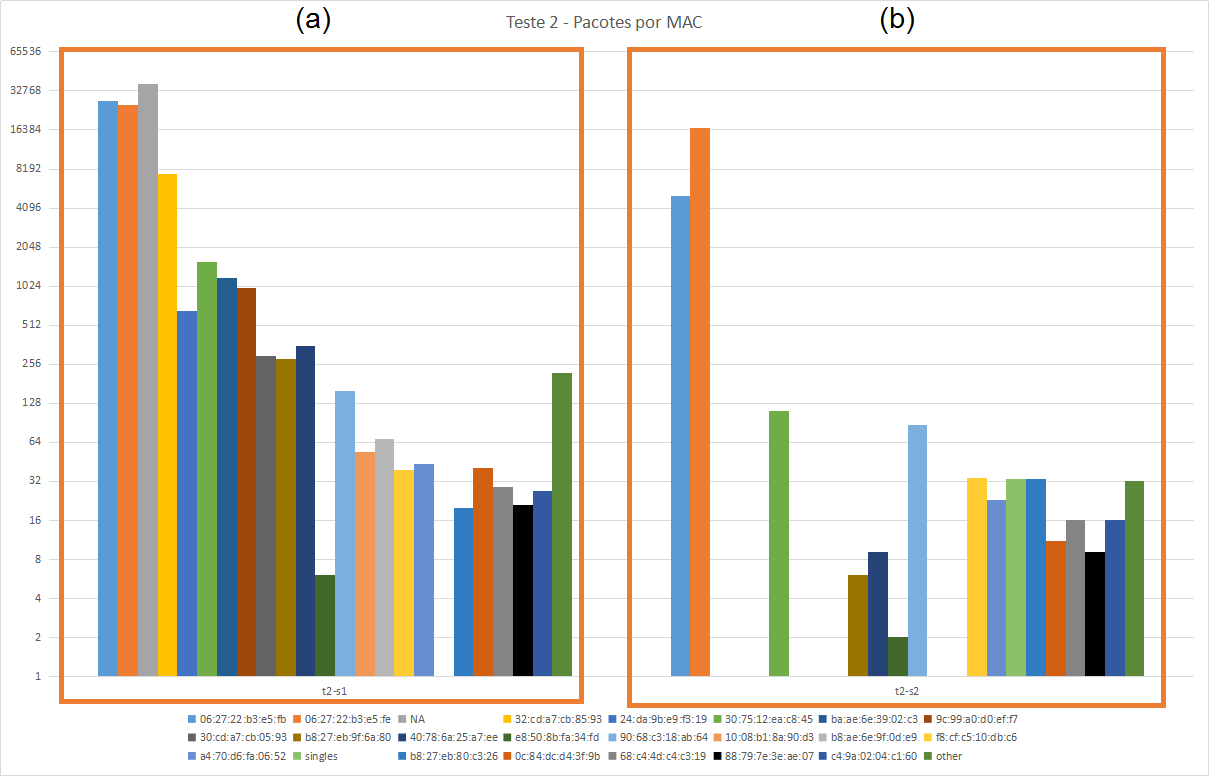
\includegraphics[width=1\textwidth]{060-testes/data-analisis/distance-mg4plus-netflix/Teste2.png}
		\legend{Fonte: Elaborada pelo autor}
	\end{minipage}
\end{figure}


\begin{figure}[htb]
	\label{mg4-distance}
	\centering
	\begin{minipage}{0.49\textwidth}
	\centering
		\caption{\label{fig-mg4-t1}dBm Motorola G4+ - Teste 1}
		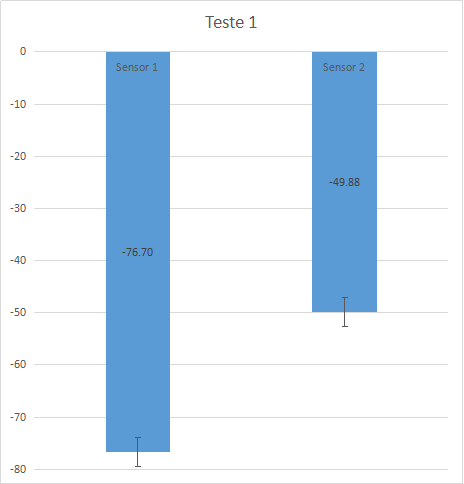
\includegraphics[width=1\textwidth]{060-testes/data-analisis/distance-mg4plus-netflix/target-Teste1.png}
		\legend{Fonte: Elaborada pelo autor}
	\end{minipage}
	\hfill
	\begin{minipage}{0.49\textwidth}
	\centering
		\caption{\label{fig-mg4-t2}dBm Motorola G4+ - Teste 2}
		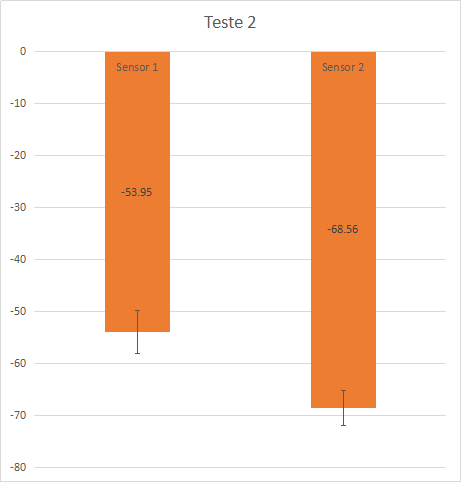
\includegraphics[width=1\textwidth]{060-testes/data-analisis/distance-mg4plus-netflix/target-Teste2.png}
		\legend{Fonte: Elaborada pelo autor}
	\end{minipage}
\end{figure}
